\documentclass[xetex,mathserif]{beamer}

\usetheme{Rochester}
\setbeamertemplate{footline}[page number]{}
\setbeamertemplate{navigation symbols}{}


\definecolor{headline_bg}{HTML}{272822}
\definecolor{headline_fg}{HTML}{66D9EF}
\setbeamercolor{headline}{bg=headline_bg,fg=headline_fg}
\setbeamercolor*{frametitle}{parent=headline}

\usepackage[frenchb]{babel}
\usepackage[latin1]{inputenc}

\usepackage{xltxtra}

\usepackage[T1]{fontenc}
\usepackage{inconsolata}
\usepackage{xparse}
\usepackage{soul}
\usepackage{xcolor}



\usepackage{listings}
\usepackage{hyperref}

\definecolor{code}{HTML}{333390}
\definecolor{badcodecolor}{HTML}{7F0000}
\definecolor{comment}{HTML}{006400}
\setstcolor{red}

\newcounter{QC}

\lstset{language=C++,
        escapeinside={(*@}{@*)},
        basicstyle=\ttfamily\color{code}\small,
        commentstyle=\color{comment},
        showstringspaces=false,
        extendedchars=true,
        breaklines=true,
        showtabs=false,
        showspaces=false,
        showstringspaces=false,
        columns=fullflexible,
        literate={\~}{{\fontfamily{ptm}\selectfont\texttildelow}}1,
        literate={\&\&}{{\textcolor{violet}{\textbf{\&\& }}}}1
        }
\lstdefinestyle{badcode}{
	basicstyle=\ttfamily\color{badcodecolor}\small,
} 

\title{Modern C++ et gestion des ressources}
\author{Corentin Jabot}
\date{Mai \st{2015} 2016 }

\begin{document}
\NoAutoSpacing

\begin{frame}
\titlepage
\end{frame}


\begin{frame}
\frametitle{C++ ?}
\begin{figure}
  Bjarne Stroustrup
  \makebox[\textwidth]{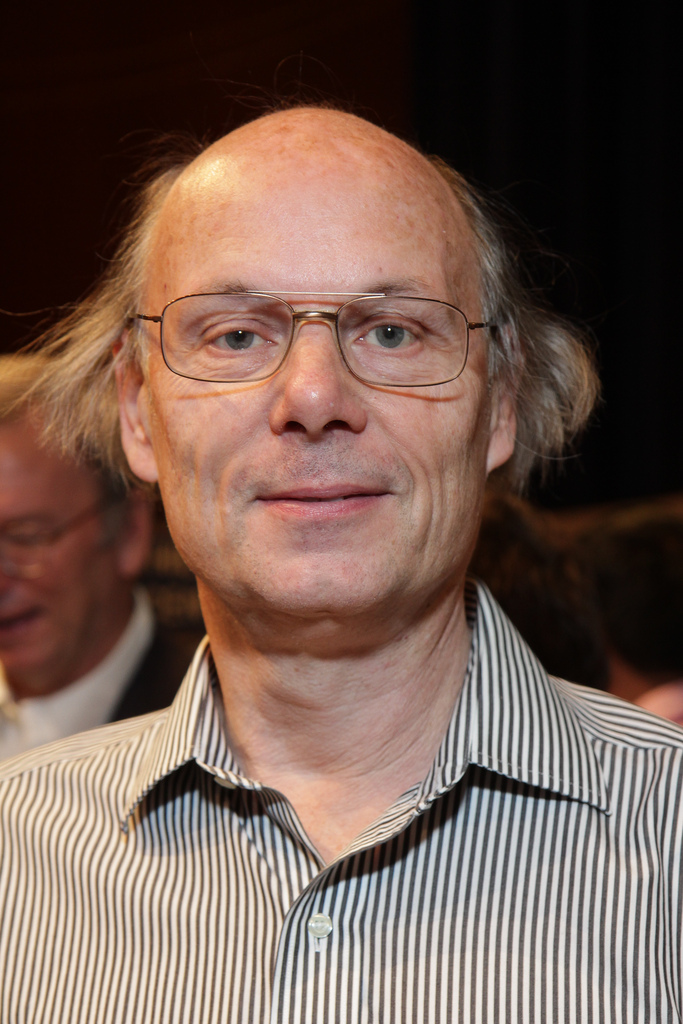
\includegraphics[height={0.7\paperheight}]{bjarne.jpg}}
\end{figure}
\end{frame}


\begin{frame}
\frametitle{C++ ?}
\begin{columns}[T]
\column{0.5\textwidth}
 \begin{itemize}
 	\onslide<1->
	 \item 1983 : "C with classes"
	 \onslide<2->
	 \item 1989 : C89
	 \onslide<3->
	 \item 1998 : C++98
	 \onslide<5->
	 \item ...
	 \onslide<4->
	 \item 2011 : C++11
\end{itemize}
\onslide<1->
\column{0.5\textwidth}
\begin{figure}
	\includegraphics<1>[width=1\textwidth]{pdp11-2.jpg}
	\includegraphics<2>[width=1\textwidth]{ps2.jpg}
	\includegraphics<3>[width=1\textwidth]{packardbell.png}
	\includegraphics<4>[width=1\textwidth]{nexus.png}
\end{figure}
\end{columns}
\end{frame}

\begin{frame}
\frametitle{C++ ?}
\begin{itemize}
	 \item Conçu pour les applications exigantes
	 \item Facilités d'abstraction
	 \item Mature, stable
\end{itemize}
\begin{itemize}
	 \item ... Compliqué
	 \item ... "Not everything to everybody"
\end{itemize}
\end{frame}

\begin{frame}
\frametitle{C++ ?}
\begin{columns}[T]
\column{0.5\textwidth}
 \begin{itemize}
	 \item Large Hadron Collider
	 \item Photoshop
	 \item Curiosity Rover
	 \item Google (Back End)
	 \item Java, PHP, Javascript, Web Renderer
	 \item Jeux, VR
\end{itemize}
\column{0.5\textwidth}
\begin{figure}
	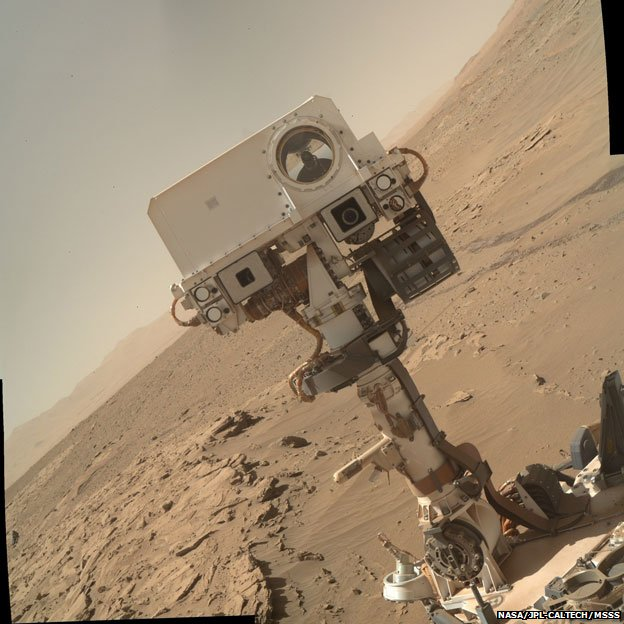
\includegraphics[width=1\textwidth]{curiosity.jpg}
\end{figure}
\end{columns}
\end{frame}

\begin{frame}
\frametitle{Evolution de C++}
\begin{itemize}
	 \item C++11 est la première version majeure depuis C++98
	 \item Toujours compatible avec le code écrit dans les années 90
	 \item Aucune feature supprimée, mais de nouvelles bonnes pratiques
	 \item Affinement de la même philosophie et des mêmes objectifs
	 \item Nombreuses nouvelles fonctionnalités
	 \item C++ continue d'evoluer : C++14, C++17, C++19...
\end{itemize}
\end{frame}

\begin{frame}
\frametitle{Question Time}
\huge Question \stepcounter{QC} \arabic{QC}
\end{frame}

\begin{frame}
\frametitle{Retour aux bases !}
\begin{itemize}
	\item \lstinline{Point a(0,1);}
		\onslide<2->
		\begin{itemize}
			\item \lstinline{Point(int, int);}
		\end{itemize}
	\onslide<3->
	\item \lstinline{Point a = Point(0,1);}
		\begin{itemize}
			\onslide<4->
			\item \lstinline{Point(int, int);}
			\onslide<5->
			\item \lstinline{Point(const Point&)}
		\end{itemize}
	\onslide<6->
	\item \lstinline{Point b = a;}
		\begin{itemize}
			\onslide<7->
			\item \lstinline{Point(const Point &);}
		\end{itemize}
	\onslide<8->
	\item \lstinline{b = a;}
		\begin{itemize}
			\onslide<9->
			\item \lstinline{Point::operator=(const Point &);}
		\end{itemize}
	\onslide<10->
	\item \lstinline{Point a = \{0, 1\};}
		\begin{itemize}
			\onslide<11->
			\item \lstinline{Point(int, int);}
		\end{itemize}
\end{itemize}
\end{frame}

\begin{frame}
\frametitle{Question Time}
\huge Question \stepcounter{QC} \arabic{QC}
\end{frame}

\begin{frame}[containsverbatim]
\frametitle{Retour aux bases !}
\begin{lstlisting}
Point midpoint(Point a, Point b) {
	return Point (
		(a.x() + b.x()) / 2,
		(a.y() + b.y()) / 2
	);
}
Point a(0, 0);
Point b(84, 84);
Point c = midpoint(a, b);
\end{lstlisting}
\end{frame}

\begin{frame}[containsverbatim]
\frametitle{Retour aux bases !}
\begin{lstlisting}
Point midpoint(const Point & a, const Point & b) {
	return Point (
		(a.x() + b.x()) / 2,
		(a.y() + b.y()) / 2
	);
}
Point a(0, 0);
Point b(84, 84);
Point c = midpoint(a, b);
\end{lstlisting}
\end{frame}

\begin{frame}
\frametitle{std::dynarray}

\begin{itemize}
	\item (futur) conteneur standard
	\pause
	\item Allocation dynamique à la construction de l'objet
	\pause
	\item Non redimensionnable
	\pause
	\item Eléments alloués et initialisés à la construction de l'objet
\end{itemize}  
\end{frame}

\begin{frame}[containsverbatim]
\frametitle{std::dynarray}
\begin{lstlisting}
	std::dynarray<std::string> bondMovies(24);
	bondMovies[0]  = "Dr. No";
	//...
	bondMovies[23] = "Spectre";
	
	std::cout << bondMovies.at(0) << bondMovies.size();  
\end{lstlisting}
\end{frame}


\begin{frame}[containsverbatim]
\frametitle{std::dynarray}
\begin{lstlisting}

template <typename T>
class dynarray {
public:
	dynarray(std::size_t);	
	std::size_t size() const;
	const T & operator[](std::size_t index) const;
	T & operator[](std::size_t index);
};
\end{lstlisting}
\end{frame}

\begin{frame}[containsverbatim]
\frametitle{std::dynarray}
\begin{lstlisting}

template <typename T>
class dynarray {
public:
	dynarray(std::size_t);	
	std::size_t size() const;
	const T & operator[](std::size_t index) const;
	T & operator[](std::size_t index);
private:
	//???????
};
\end{lstlisting}
\end{frame}

\begin{frame}
\frametitle{Question Time}
\huge Question \stepcounter{QC} \arabic{QC}
\end{frame}


\begin{frame}[containsverbatim]
\frametitle{std::dynarray}
\begin{lstlisting}

template <typename T>
class dynarray {
public:
	dynarray(std::size_t);	
	std::size_t size() const;
	const T & operator[](std::size_t index) const;
	T & operator[](std::size_t index);
private:
	T* m_data;
	std::size_t m_size;
};
\end{lstlisting}
\end{frame}

\begin{frame}
\frametitle{Question Time}
\huge Question \stepcounter{QC} \arabic{QC}
\end{frame}

\begin{frame}[containsverbatim]
\frametitle{std::dynarray}
\begin{lstlisting}

template <typename T>
dynarray<T>::dynarray(std::size_t size)
	: m_data(new T[size])
	, m_size(size) {	
}

\end{lstlisting}
\end{frame}


\begin{frame}[containsverbatim]
\frametitle{std::dynarray}
\begin{lstlisting}

template <typename T>
class dynarray {
public:
	dynarray(std::size_t);
	~dynarray();
	std::size_t size() const;
	const T & operator[](std::size_t index) const;
	T & operator[](std::size_t index);
private:
	T* m_data;
	std::size_t m_size;
};
\end{lstlisting}
\end{frame}

\begin{frame}[containsverbatim]
\frametitle{std::dynarray}
\begin{lstlisting}

template <typename T>
dynarray<T>::dynarray(std::size_t size)
	: m_data(new T[size])
	, m_size(size) {	
}

template <typename T>
dynarray<T>::~dynarray() {
	delete[] m_data;	
}


\end{lstlisting}
\end{frame}

\begin{frame}
\frametitle{Question Time}
\huge Question \stepcounter{QC} \arabic{QC}
\end{frame}

\begin{frame}[containsverbatim]
\frametitle{std::dynarray}
\framesubtitle{Règle de 3}
\begin{lstlisting}

template <typename T>
class dynarray {
public:
	dynarray(std::size_t);
	~dynarray();
	
	//...
};
\end{lstlisting}
\end{frame}

\begin{frame}[containsverbatim]
\frametitle{std::dynarray}
\framesubtitle{Règle de 3}
\begin{lstlisting}

template <typename T>
class dynarray {
public:
	dynarray(std::size_t);
	~dynarray();
	
	dynarray(const dynarray<T> & other);
	
	//...
};
\end{lstlisting}
\end{frame}

\begin{frame}[containsverbatim]
\frametitle{std::dynarray}
\framesubtitle{Règle de 3}
\begin{lstlisting}

template <typename T>
class dynarray {
public:
	dynarray(std::size_t);
	~dynarray();
	
	dynarray(const dynarray<T> & other);
	dynarray& operator=(const dynarray<T> & other);
	
	//...
};
\end{lstlisting}
\end{frame}


\begin{frame}[containsverbatim]
\frametitle{std::dynarray}
\framesubtitle{Règle de 3}

Comportements des méthodes de copie générées par le compilateur

\begin{lstlisting}[style=badcode]
template <typename T>
dynarray<T>::dynarray(const dynarray<T> & other)
	: m_data(other.m_data)
	, m_size(other.m_size) { 
}

\end{lstlisting} \begin{lstlisting}
void f() {
	dynarray<int> a(42);
	dynarray<int> b = a;
}
\end{lstlisting}


\end{frame}



\begin{frame}[containsverbatim]
\frametitle{std::dynarray}
\framesubtitle{Règle de 3}
\begin{lstlisting} 

template <typename T>
dynarray<T>::dynarray(const dynarray<T> & other)
	: m_data(new T[other.m_size])
	, m_size(other.m_size) {
	
	for(std::size_t i = 0; i < m_size; ++i) {
		m_data[i] = other.m_data[i];
	}
}
\end{lstlisting}
\end{frame}


\begin{frame}[containsverbatim]
\frametitle{std::dynarray}
\framesubtitle{Règle de 3}
\begin{lstlisting} 
template <typename T>
dynarray<T> & dynarray<T>::operator=(const dynarray<T> & other) {

	if(this == &other)
		return *this;
	
	delete[] m_data;
	
	m_data = new T[other.m_size];
	m_size = other.m_size;
	
	for(std::size_t i = 0; i < m_size; ++i) {
		m_data[i] = other.m_data[i];
	}
	
	return *this;
}
\end{lstlisting}
\end{frame}

\begin{frame}[containsverbatim]
\frametitle{std::dynarray}
\framesubtitle{Règle de 3}

\begin{lstlisting} 

	dynarray<int> a(1337);
	dynarray<int> b(42);	
	//...
	a = b;

\end{lstlisting}
\end{frame}



\begin{frame}[fragile]
\frametitle{std::dynarray}
\framesubtitle{Règle de 3}

On veut pouvoir empêcher la copie, ou l'assignement par copie de certains type....
\begin{lstlisting}
dynarray& operator=(const dynarray<T> & other) = delete;
\end{lstlisting}

\pause
... Ou demander explicitement au compilateur de générer un opérateur par défaut

\begin{lstlisting}
Point(const Point<T> & other) = default;
\end{lstlisting}

\end{frame}


\begin{frame}[containsverbatim]
\frametitle{std::dynarray}
\framesubtitle{Règle de 3}
\begin{lstlisting}

template <typename T>
class dynarray {
public:
	dynarray(std::size_t);
	~dynarray();
	dynarray(const dynarray<T> & other);
	dynarray& operator=(const dynarray<T> &) = delete;
	std::size_t size() const;
	const T & operator[](std::size_t index) const;
	T & operator[](std::size_t index);
private:
	T* m_data;
	std::size_t m_size;
};
\end{lstlisting}
\end{frame}


\begin{frame}[containsverbatim]
\frametitle{Règle de 3}
A retenir
\begin{itemize}
	\item l'implémentation d'un destructeur, constructeur par copie ou opérateur d'assignement par copie, dénote d'une gestion non triviale d'une
	ou plusieurs variables membres.
	\item Règle de 3 : Définir
		\begin{itemize} 
			\item Destructeur
			\item Constructeur par copie
			\item Opérateur d'assignement par copie
	 	\end{itemize}
	 \item Forcer le compilateur à générer une méthode par défaut avec \lstinline{ = default;}
	 \item Empêcher le compilateur de générer une méthode par défaut avec \lstinline{ = delete;}
\end{itemize}
\end{frame}

\begin{frame}
\frametitle{Question Time}
\huge Question \stepcounter{QC} \arabic{QC}
\end{frame}

\begin{frame}[fragile]
\frametitle{Retourner par valeur}
\begin{lstlisting}
dynarray<std::string> collectNames() {
	
    std::size_t size = 1'000'000;
    dynarray<std::string> names(size);
    //...
    return names;
}

void foo() {
    dynarray<std::string> names = collectNames();
}
\end{lstlisting}
\begin{itemize} 
	\pause
	\item 2 000 000 instances de \lstinline{std::string} lors de la copie
	\pause
	\item 3 000 0000 instances crées puis détruites dans la durée de vie du programme ( en ignorant les optimisation du compilateur)
	\pause
	\item => Performances désastreuses
\end{itemize}
\end{frame}


\begin{frame}[fragile]
\frametitle{Retourner par valeur}

\begin{lstlisting}[style=badcode]
dynarray<std::string>* collectNames() {
	
    std::size_t size = 1'000'000;
    dynarray<std::string>* names
        = new dynarray<std::string>(size);
    //...
    return names;
}

void foo() {
    dynarray<std::string>* names = collectNames();
    delete names;
}
\end{lstlisting}
\pause
\begin{center}
\huge NOPE.
\end{center}
\end{frame}

\begin{frame}[fragile]
\frametitle{Retourner par valeur}

\begin{lstlisting}[style=badcode]
collectNames(dynarray<std::string> & result) {
	
    std::size_t size = 1'000'000;
    dynarray<std::string> names;
    //...
    result = names;
}
\end{lstlisting}
\pause
\begin{lstlisting}[style=badcode]
void foo() {
    dynarray<std::string> names(????);
    collectNames(names);
}
\end{lstlisting}
\end{frame}


\begin{frame}[fragile]
\frametitle{Retourner par valeur}
\begin{lstlisting}[style=badcode]
collectNames(dynarray<std::string> & result) {
	
    std::size_t size = 1'000'000;
    dynarray<std::string> names;
    //...
    result = names; //Ne compile pas ( souvenez vous, operator=  déclaré "=delete");
}
void foo() {
    dynarray<std::string> names(????);
    collectNames(names);
}
\end{lstlisting}
\end{frame}



\begin{frame}[fragile]
\frametitle{Retourner par valeur}

\begin{itemize} 
	\item Retourner par pointeur : Pas élégant, peu compréhensible, très dangereux.
	\pause
	\item Paramètre de sortie ( référence) : pas toujours possible, pas intuitif non plus.
	\pause
	\item Retourner par valeur : simple, mais création de copies...
\end{itemize}
\pause
A moins que...
\end{frame}


\begin{frame}[fragile]
\frametitle{Sémantique de Déplacement ( move )}
\begin{itemize} 
	\item Beaucoup de copies sont suivies de destruction ( retour de fonction )
	\pause
	\item Selon le niveau d'optimisation le compilateur peut éliminer certaines copies de valeur de retour ( RVO )
	\pause
	\item La majorité des classes encapsulent des données allouées dynamiquement
\end{itemize}
\end{frame}

\begin{frame}[fragile]
\frametitle{Sémantique de Déplacement ( move )}
\begin{itemize} 
	\item Solution: \textbf{déplacer} les variables membres dans le cas ou l'objet va être détruit (C++11)
	\pause
	\item Le compilateur sait détecter les variables sur le point d'être détruites
	\pause
	\item Il est possible de créer des Constructeur par copie et des opérateurs d'assignement spécifiques pour ce cas de figure.
\end{itemize}
\end{frame}


\begin{frame}[containsverbatim]
\frametitle{Sémantique de Déplacement ( move )}
\begin{lstlisting}

template <typename T>
class dynarray {
public:
	dynarray(std::size_t);
	~dynarray();
	dynarray(const dynarray<T> & other);
	dynarray& operator=(const dynarray<T> &) = delete;
	
	
	//! Constructeur par déplacement
	dynarray(dynarray<T> && other); 
	
	//! operateur d'assignement par déplacement
	dynarray& operator=(dynarray<T> && other) = delete;
	
	//..
};
\end{lstlisting}
\end{frame}


\begin{frame}[containsverbatim]
\frametitle{Sémantique de Déplacement ( move )}
\begin{lstlisting} 
template <typename T>
dynarray<T>::dynarray(dynarray<T> && other)
	: m_data(other.m_data)
	, m_size(other.m_size) {
	
	other.m_data = 0;
}

template <typename T>
dynarray<T> & dynarray<T>::operator=(dynarray<T> && other) {

	std::swap(m_data, other.m_data);
	std::swap(m_size, other.m_size);
}
\end{lstlisting}
\end{frame}


\begin{frame}[fragile]
\frametitle{Sémantique de Déplacement ( move )}
A retenir

\begin{itemize} 
	\item En C++11, retourner de gros objets est performant et recommandé
	\item Le compilateur sait distinguer les variables qui peuvent être déplacées de celles qui doivent être copiées
	\item Déplacement = Optimisation de la copie
	\item 2 nouvelles "fonction spéciales" : La règle de 3 devient règle de 5.
	\item Introduction au sujet, à vous d'approfondir...
		
\end{itemize}
\end{frame}



\begin{frame}[fragile]
\frametitle{Gestion des ressources}
\begin{itemize}
	\pause
	\item Une ressource désigne tout ce qui peut être mis à disposition du programme par le système d'exploitation ou le matériel sous-jacent.
	\pause
	\item Acquérir / Libérer
	\pause
	\item Exemples:
	\begin{itemize}
		\item Fichier  \lstinline{ open / close }
		\item Bloc mémoire  \lstinline{ new / delete }
		\item Socket réseau \lstinline{ connect / close }
		\item Le bras du robot Curiosity, une fenêtre d'application, une imprimante, etc
	\end{itemize}
	\pause
	\item Les ressources sont rares	
	\pause 
	\item \large Les ressources acquise doivent toujours être libérées!	 
\end{itemize}
\end{frame}


\begin{frame}[fragile]
\frametitle{Gestion des ressources}
\begin{lstlisting}[style=badcode] 
bool fileStartsWithA(const char* filename) {
    FILE* file = open(filename, "r");
    if(!file)
    	return false;

    unsigned char buffer;
    if(fread(&buffer, 1, 1, file) == 0 )
    	return false;

    if(buffer == 'A')
        return true;
        
    close(file); 
    return false;
}
\end{lstlisting}
\end{frame}

\begin{frame}[fragile]
\frametitle{Resource Acquisition Is Initialization}
\framesubtitle{l'Acquisition d'une Ressource est une Initialisation}
\begin{itemize}
	\item Technique de gestion des ressources en C++
	\item Mise au point en 1984
	\item Reprise récemment par Rust \& D
	\item La ressource est acquise dans le constructeur, et libérée dans le destructeur
	\item Généralisation : la ressource est libérée dans le destructeur
\end{itemize}
\end{frame}


\begin{frame}[fragile]
\frametitle{Resource Acquisition Is Initialization}
\framesubtitle{l'Acquisition d'une Ressource est une Initialisation}

La classe \lstinline{dynarray} est un bon exemple de RAII

\begin{lstlisting}
template <typename T>
dynarray<T>::dynarray(std::size_t size)
    : m_data(new T[size])
    , m_size(size) {	
}

template <typename T>
dynarray<T>::~dynarray() {
    delete[] m_data;	
}
\end{lstlisting}
\end{frame}

\begin{frame}
\frametitle{Question Time}
\huge Question \stepcounter{QC} \arabic{QC}
\end{frame}

\begin{frame}[fragile]
\frametitle{Resource Acquisition Is Initialization}
\framesubtitle{l'Acquisition d'une Ressource est une Initialisation}
Les classes de la librairies standard implémentent également ce principe:
\begin{itemize}
	\item \lstinline{std::vector}
	\item \lstinline{std::string}
	\item \lstinline{fstream}
\end{itemize}
\end{frame}

\begin{frame}
\frametitle{Question Time}
\huge Question \stepcounter{QC} \arabic{QC}
\end{frame}

\begin{frame}[fragile]
\frametitle{Resource Acquisition Is Initialization}
\framesubtitle{l'Acquisition d'une Ressource est une Initialisation}
\begin{lstlisting} 
class File {
    FILE* handle;
	
public:
    File(const char* filename, const char* mode)  {
       handle = open(filename, mode);
    }
    
    ~File() {
        close(handle);
    }
    
    File(const File & other) = delete;
    File & operator=(const File & file) = delete;
};
\end{lstlisting}
\end{frame}


\begin{frame}
\frametitle{Question Time}
\huge Question \stepcounter{QC} \arabic{QC}
\end{frame}


\begin{frame}[fragile]
\frametitle{Resource Acquisition Is Initialization}
\framesubtitle{l'Acquisition d'une Ressource est une Initialisation}
\begin{lstlisting}

Shape* shapeFromName(const std::string & name ) {
    if(name == "square")
        return new Square;
    if(name == "triangle")
        return new Triangle;
    return nullptr;
}

void f() {
    Shape* shape = shapeFromName("triangle");
}
\end{lstlisting}
\end{frame}


\begin{frame}[fragile]
\frametitle{Resource Acquisition Is Initialization}
\framesubtitle{l'Acquisition d'une Ressource est une Initialisation}
\begin{lstlisting}

Shape* shapeFromName(const std::string & name ) {
    if(name == "square")
        return new Square;
    if(name == "triangle")
        return new Triangle;
    return nullptr;
}

void f() {
    Shape* shape = shapeFromName("triangle");
    delete shape;
}
\end{lstlisting}
\end{frame}


\begin{frame}[fragile]
\frametitle{Smart pointers}
\framesubtitle{Pointeurs intelligents}

\begin{itemize}
	\item Classes qui permettent la gestion automatique de la durée de vie d'une ressource allouée sur le tas
	\item Basées sur le principe de RAII
	\item header \lstinline{<memory>}
	\begin{itemize}
		\item \lstinline{std::unique_ptr} : Non copiable
		\item \lstinline{std::shared_ptr} : Partagé, copiable ( l'objet est détruit lorsque toutes les copies  sont détruites)
		\item \lstinline{std::weak_ptr} : Construit à partir d'un \lstinline{std::shared_ptr}, permet d'"observer" un pointeur sans influencer sur sa durée de vie 
	\end{itemize}
\end{itemize}
\end{frame}


\begin{frame}[fragile]
\frametitle{Smart pointers}
\framesubtitle{Pointeurs intelligents}

\begin{lstlisting}
{
    std::unique_ptr<Shape> shape(new Triangle);
    std::cout << shape->name() << std::endl;
}
\end{lstlisting}
\pause
\begin{lstlisting}
{
    std::shared_ptr<Shape> shape(new Triangle);
    std::shared_ptr<Shape> copy = shape;
}
\end{lstlisting}

\end{frame}


\begin{frame}[fragile]
\frametitle{Smart pointers}
\framesubtitle{Pointeurs intelligents}

\begin{lstlisting}
{
    std::unique_ptr<Shape> shape 
        = std::make_unique<Triangle>();
    
    std::cout << shape->name() << std::endl;
}
\end{lstlisting}

\begin{lstlisting}
{
    std::shared_ptr<Shape> shape 
        = std::make_shared<Triangle>();
    
    std::shared_ptr<Shape> copy = shape;
}
\end{lstlisting}
\end{frame}

\begin{frame}[fragile]
\frametitle{Smart pointers}
\framesubtitle{Pointeurs intelligents}

\begin{lstlisting}
{
    auto shape  = std::make_unique<Triangle>();
    std::cout << shape->name() << std::endl;
}
\end{lstlisting}

\begin{lstlisting}
{
    auto shape  = std::make_shared<Triangle>();
    std::shared_ptr<Shape> copy = shape;
}
\end{lstlisting}
\end{frame}


\begin{frame}[fragile]
\frametitle{Smart pointers}
\framesubtitle{Pointeurs intelligents}

Principales fonctionnalités:
\begin{lstlisting}
std::unique_ptr<Shape> shape  = std::make_unique<Triangle>();

//accès aux membres de l'objet géré par le pointeur
std::cout << shape->name() << std::endl;

//Récupération du pointeur
Shape& ptr  = *ptr;
Shape* ptr2 = ptr.get();

//tester si le pointeur est nul
if(!shape) {
	// le pointeur est null
}
\end{lstlisting}
\end{frame}

\begin{frame}
\frametitle{Question Time}
\huge Question \stepcounter{QC} \arabic{QC}
\end{frame}

\begin{frame}[fragile]
\frametitle{Smart pointers}

\begin{lstlisting}
std::unique_ptr<Shape>
shapeFromName(const std::string & string ) {
    if(string == "square")
        return make_unique<Square>();
    if(string == "triangle")
        return make_unique<Triangle>();
    return std::unique_ptr<Shape>();
}
\end{lstlisting}
\pause
\begin{lstlisting}
void f() {
    std::unique_ptr<Shape> shape = shapeFromName("triangle");
}
\end{lstlisting}
\end{frame}

\begin{frame}
\frametitle{Question Time}
\huge Question \stepcounter{QC} \arabic{QC}
\end{frame}


\begin{frame}[fragile]
\frametitle{Smart pointers}

\begin{lstlisting}

std::(*@\line(1,0){50}@*)<Shape> shapeFromName(const std::string &);

std:string shapeName((*@\line(1,0){50}@*)shape) {
    return shape->name();
}
void f() {
    (*@\line(1,0){50}@*) shape = shapeFromName("hello");
    std:: cout << shapeName((*@\line(1,0){50}@*)) << std::endl;
}
\end{lstlisting}
\end{frame}

\begin{frame}[fragile]
\frametitle{Smart pointers}

\begin{lstlisting}

std::unique_ptr<Shape> 
shapeFromName(const std::string &);

std:string shapeName(const Shape* shape) {
    if(!shape)
        return "";
    return shape->name();
}
void f() {
    std::unique_ptr<Shape> shape 
            = shapeFromName("hello");
    
    std::cout << shapeName(shape.get()) << std::endl;
}
\end{lstlisting}

\end{frame}

\begin{frame}
\frametitle{Question Time}
\huge Question \stepcounter{QC} \arabic{QC}
\end{frame}


\begin{frame}[fragile]
\frametitle{Smart pointers}

\begin{lstlisting}
template <typename T>
class std::unique_ptr {
    T* ptr;
public:
    unique_ptr(T*);
    ~unique_ptr();
 
    unique_ptr(const unique_ptr<T> &) = delete;
    unique_ptr(const unique_ptr<T> &&) = default;
    
    unique_ptr<T>& operator=(const unique_ptr<T> &) = delete;
    unique_ptr<T>& operator=(unique_ptr<T> &&) = default;
    
    T* operator->() const; 	
    operator bool() const;
    T & operator*() const;
    T* get() const;
};
\end{lstlisting}

\end{frame}

\begin{frame}[fragile]
\frametitle{Conclusion}

\begin{itemize}
	\item Retournez de préférence par valeur
	\item Passez les paramètes d'entrée par référence constante
	\item Utilisez le principe de RAII pour gérer les ressources système.
	\item Pensez à la règle de 3 (et 5)
	\item Préférez ne redéfinir aucun destructeur / opérateur ou constructeur de copie : \textbf{règle de 0}
\end{itemize}

\end{frame}

\begin{frame}[fragile]
\frametitle{Conclusion}

\begin{itemize}
	\item Evitez d'utiliser \lstinline{new} et \lstinline{delete} 
	\item Utilisez les smart pointers pour gérer la durée de vie des objets alloués dynamiquement
	\item Préférez \lstinline{std::make_unique} et \lstinline{std::make_shared} pour créer des pointeurs intelligents.
	\item N'utilisez de smarts pointers que lorsque vous avez besoin de gérer la durée de vie de l'objet. Continuez d'utiliser des pointeurs et des références dans les autres cas. 
\end{itemize}

\end{frame}







\end{document}